\item \points{20} {\bf AdaBoost Performance}

We learned about boosting in lecture. Statistician Kevin Murphy claims that ``It can be shown that, as long as each base learner has an accuracy that is better than chance (even on the weighted dataset), then the final ensemble of classifiers will have higher accuracy than any given component." We will now verify this in the AdaBoost framework.


\begin{enumerate}
    \item \subquestionpoints{5} Show that for any given split, the weighted Gini loss of the children can not exceed that of the parent. (\textbf{Hint}: first show that the Gini loss is strictly concave. And then use the fact that G is strictly concave meaning:
    \begin{align*}
        \forall p_1 \neq p_2, \forall t \in (0, 1): G(t p_1 + (1 - t) p_2) > t G(p_1) + (1 - t) G(p_2)
    \end{align*}
    
	\ifnum\solutions=1 {
	\begin{answer}
\end{answer}
        } \fi
        
    \item \subquestionpoints{5} A multivariate decision tree is a generalization of univariate decision trees, where more than one attribute can be used in the decision rule for each split. For the same data, learn a multivariate decision tree where each decision rule is a linear classifier that makes decisions based on the sign of $\alpha x_{\text{age}} +\beta x_{\text{income}} -1$. Provide a list of all splits with the classification error reduction at each split, as well as $\alpha$, $\beta$. For $\alpha$ and $\beta$, keep two significant decimals.


    
	\ifnum\solutions=1 {
	\begin{answer}
% Accuracy for college degree dataset: 90.0\% \\
% Accuracy for iris dataset: 93.33\% \\
\begin{figure}[H]
    \centering
    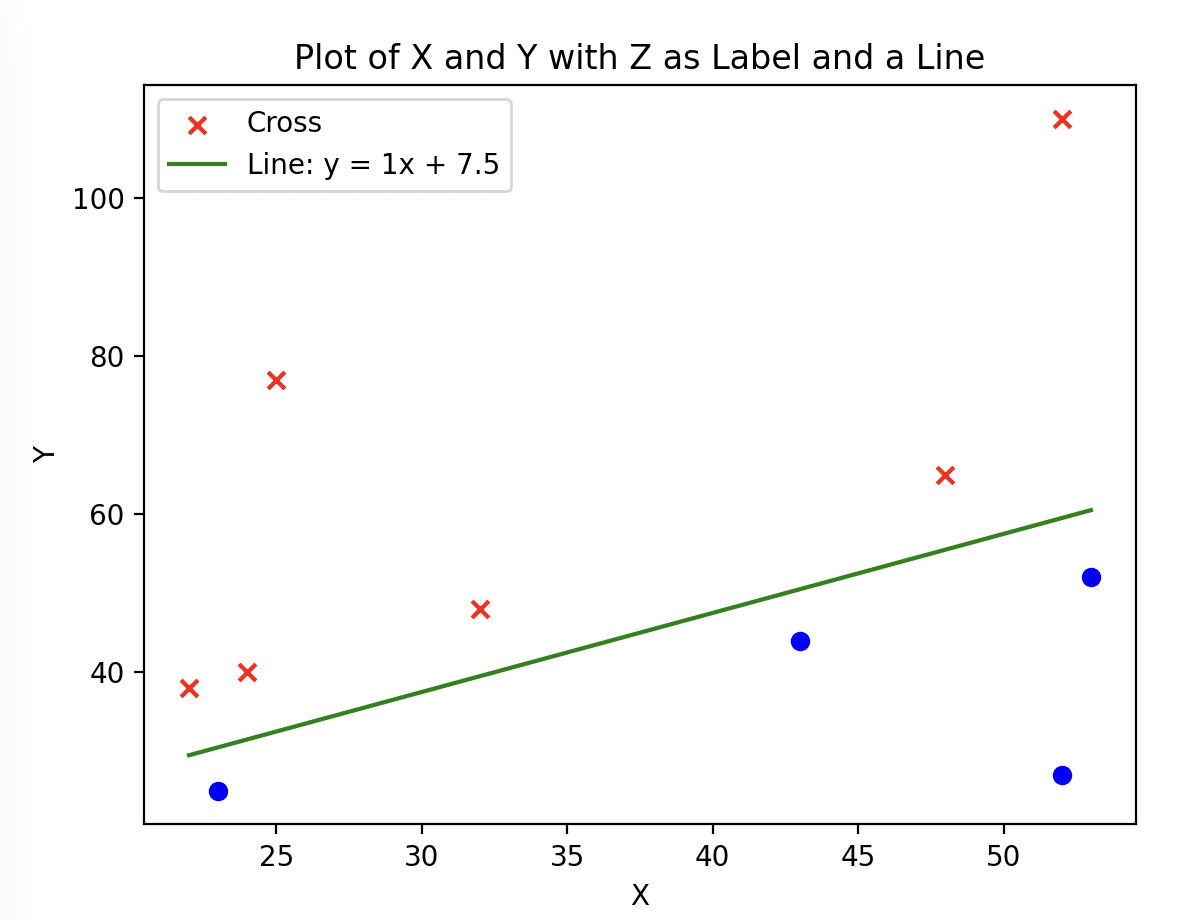
\includegraphics[width=0.5\linewidth]{Screenshot 2024-02-20 at 23.45.57.png}
    \caption{ps3::q1::c}
    \label{fig:enter-label}
\end{figure}

The above figure shows the training samples can be linearly separated by $income = age + 7.5$, this line is equivalent to 
\begin{equation}
    -0.13 \cdot  \text{age} + 0.13 \cdot  \text{income} - 1 = 0
\end{equation}

so $\alpha = -0.13$, $\beta = 0.13$. At root node the classification error is 4, and after one slipt, we get two leaf nodes with classification error = 0
\end{answer}
        } \fi
        
    \item \subquestionpoints{4} If instead we use misclassification loss, what additional case causes the loss to stay the same after a split?  Show why this is (hint: you may find it useful to define $N_m = \lvert R_m \rvert$ and $N_{mk}$ as the number of examples of class $k$ present in $R_m$).
    
	\ifnum\solutions=1 {
	\begin{answer}

Let the parent node $R_p$ have $N_p$ instances in total, with $N_{p1}$ instances of class 1 and $N_{p2}$ instances of class 2, where $N_{p1} > N_{p2}$

The misclassification loss of the parent node is:

\begin{equation}
    M(R_p) = 1 - \frac{N_{p1}}{N_p}
\end{equation}

After the Split, lets assume
\begin{itemize}
    \item \(R_1\) contains \(N_1\) instances, with \(N_{11}\) of class 1 and \(N_{12}\) of class 2.
    \item \(R_2\) contains \(N_2\) instances, with \(N_{21}\) of class 1 and \(N_{22}\) of class 2.
\end{itemize}

The weighted misclassification loss after the split is calculated as:

\begin{equation}
M_{\text{weighted}} = \frac{\lvert R_1 \rvert L(R_1) + \lvert R_2 \rvert L(R_2)}{\lvert R_1 \rvert + \lvert R_2 \rvert} = \frac{N_1 M(R_1) + N_2 M(R_2)}{N_1 + N_2} 
\end{equation}

And 
\begin{equation}
M(R_1) = 1 - \frac{\max(N_{11}, N_{12})}{N_1}
\end{equation}
\begin{equation}
M(R_2) = 1 - \frac{\max(N_{21}, N_{22})}{N_2}
\end{equation}

Replace (9), (10) into (8), and replace $M_{\text{weighted}}$ with (7), we got the the following 
\begin{equation}
\frac{N_1}{N_P}(1 - \frac{\max(N_{11}, N_{12})}{N_1}) + \frac{N_2}{N_P}(1 - \frac{\max(N_{21}, N_{22})}{N_2}) = 1 - \frac{N_{p1}}{N_p}
\end{equation}

Or equivalently, 
\begin{equation}
    N_{p1} = \max(N_{11}, N_{12}) + \max(N_{21}, N_{22})
\end{equation}

so as long as the sum of number of the most frequent classes in two children equals the number of most frequent class in parent, loss will be the same.
\end{answer}
        } \fi
        
\end{enumerate}
